\section{Architettura del sistema}

Il software è organizzato secondo un'architettura di tipo \textit{client-server}. Nelle sezioni che seguono vengono presentate nel dettaglio le componenti client e server tramite diagrammi delle classi e descrizioni testuali sulla loro struttura e funzionamento.

\begin{figure}[H]
	\centering
	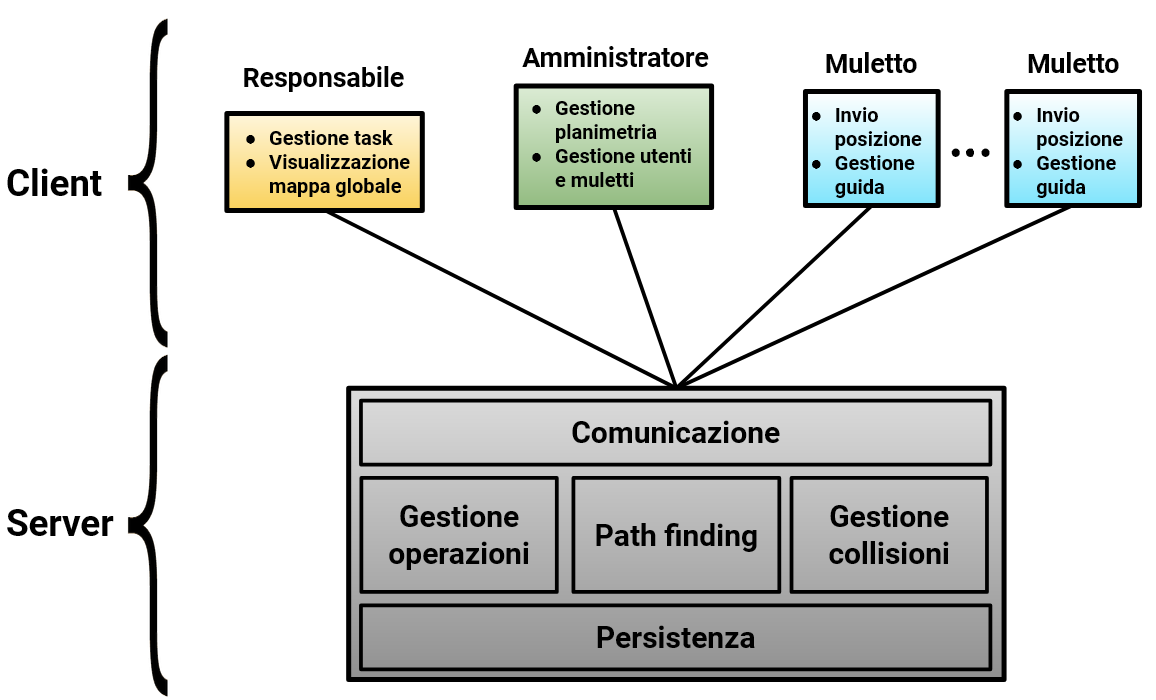
\includegraphics[scale=0.34]{res/images/architettura_complessiva.png}
	\caption{Rappresentazione ad alto livello dell'architettura del software}
\end{figure}













